\section{Introduktion}
\begin{itemize}
	\item Nice-to-have lag
	\item Sockets bruges til kommunikation med applikationslaget
	\item Laver TCP/UDP pakker med headers
	\item Multiplexing
	\item Demultiplexing
\end{itemize}

{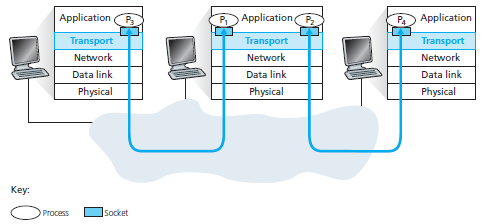
\includegraphics{3-transport-layer/transport-layer-sockets.png}

\section{TCP}
\begin{itemize}
	\item Transmission Control Protocol
	\item Connection orienteret
	\item 3-way-handshake
	\item Maksimal pakkestørrelse på64 kBytes, men bruger som regel 1500 bytes
	\item Identificeres ved et socket par (IP1:80,IP1:81)
	\item Bytestream
	\item Pålidelig
	\item Flow control
	\item Congestion handling
\end{itemize}

{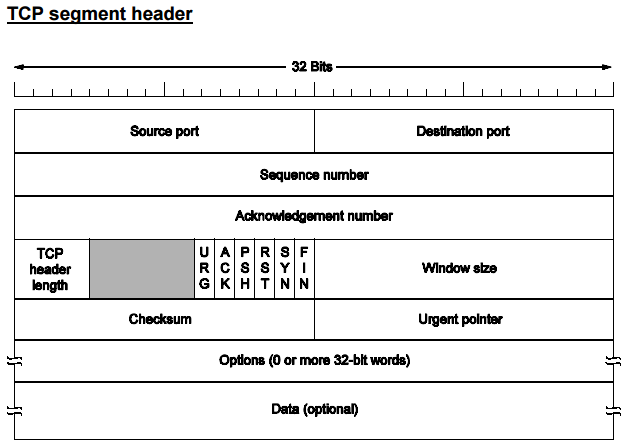
\includegraphics{3-transport-layer/tcp-header.png}

\section{UDP}
\begin{itemize}
	\item User Datagram Protocol
	\item Connection-less
	\item Ip datagram med en lille UDP header
	\item Upålidelig
\end{itemize}

{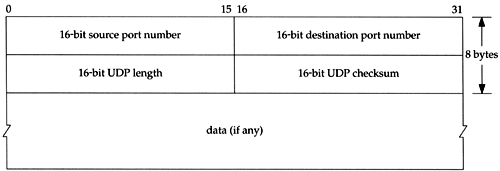
\includegraphics{3-transport-layer/udp-header.png}

\section{Brug af protokoller}

{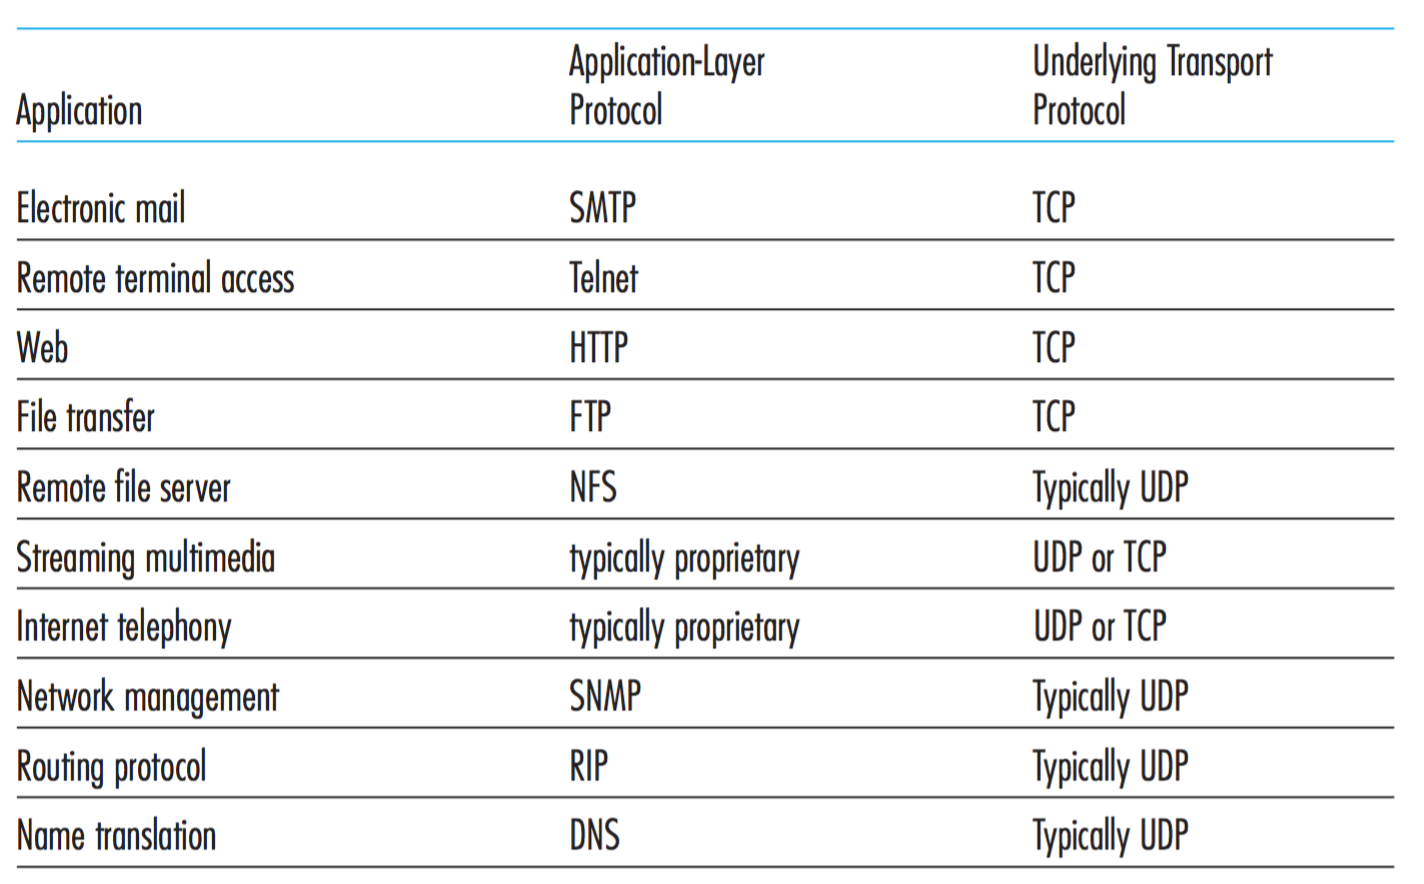
\includegraphics[scale=0.6]{3-transport-layer/brug-af-protokoller.png}